\documentclass[11pt]{article}
\usepackage[margin=0.85in]{geometry}
\usepackage{amsmath,amssymb,amsfonts,mathtools,bm}
\usepackage{booktabs,longtable,array,multirow}
\usepackage{hyperref}
\usepackage{xcolor}
\usepackage{enumitem}
\usepackage{graphicx}
\usepackage{listings}
\usepackage{caption}
\usepackage{fancyhdr}
\usepackage{titlesec}
\usepackage{tikz}
\usetikzlibrary{arrows.meta,positioning,fit,calc,shapes.geometric,backgrounds,matrix,decorations.pathreplacing}
\hypersetup{colorlinks=true,linkcolor=blue,citecolor=blue,urlcolor=blue}
\pagestyle{fancy}
\setlength{\headheight}{14pt}
\fancyhf{}
\lhead{NeuroTwin NFC Research Constitution}
\rhead{Draft for coding discipline}
\cfoot{\thepage}
\setlist[itemize]{topsep=2pt,itemsep=2pt,parsep=2pt}
\setlist[enumerate]{topsep=2pt,itemsep=2pt,parsep=2pt}
\titleformat{\section}{\Large\bfseries}{\thesection}{1em}{}
\titleformat{\subsection}{\large\bfseries}{\thesubsection}{1em}{}
\titleformat{\subsubsection}{\normalsize\bfseries}{\thesubsubsection}{1em}{}
\lstset{basicstyle=\ttfamily\small,breaklines=true,frame=single,backgroundcolor=\color{gray!5}}

% Nature/AlphaFold-inspired visual grammar for original NeuroTwin schematics.
% These figures are original diagrams; they do not reproduce AlphaFold artwork.
\definecolor{nfcBlue}{RGB}{20,74,168}
\definecolor{nfcLightBlue}{RGB}{204,226,243}
\definecolor{nfcOrange}{RGB}{237,125,49}
\definecolor{nfcLightOrange}{RGB}{252,221,201}
\definecolor{nfcGreen}{RGB}{76,153,80}
\definecolor{nfcLightGreen}{RGB}{218,238,218}
\definecolor{nfcPurple}{RGB}{112,88,170}
\definecolor{nfcLightPurple}{RGB}{230,224,245}
\definecolor{nfcGray}{RGB}{90,90,90}
\newcommand{\panel}[1]{\textbf{\large #1}\,}
\newcommand{\claimbox}[1]{\vspace{0.4em}\noindent\fbox{\begin{minipage}{0.95\linewidth}#1\end{minipage}}\vspace{0.4em}}


\title{\Huge NeuroTwin NFC: A Neural Field Compiler for Brain Dynamics\\[0.5em]
\Large Mathematical, Computer-Science, and Research-Process Constitution}
\author{Internal Research Draft for NeuroTwin Coding Discipline}
\date{\today}

\newcommand{\R}{\mathbb{R}}
\newcommand{\E}{\mathbb{E}}
\newcommand{\KL}{\mathrm{KL}}
\newcommand{\tr}{\mathrm{tr}}
\newcommand{\softmax}{\operatorname{softmax}}
\newcommand{\diag}{\operatorname{diag}}
\newcommand{\rank}{\operatorname{rank}}
\newcommand{\Cov}{\operatorname{Cov}}
\newcommand{\Var}{\operatorname{Var}}
\newcommand{\N}{\mathcal{N}}
\newcommand{\Poisson}{\operatorname{Poisson}}
\newcommand{\MI}{\operatorname{I}}
\newcommand{\loss}{\mathcal{L}}
\newcommand{\Obs}{\mathcal{O}}
\newcommand{\Infer}{\mathcal{I}}
\newcommand{\Field}{\mathcal{F}}
\newcommand{\Graph}{\mathcal{G}}
\newcommand{\Operator}{\mathcal{G}_\theta}
\newcommand{\todo}[1]{\textcolor{red}{\textbf{TODO:} #1}}

\begin{document}
\maketitle

\begin{abstract}
This document is a deliberately large, mathematics-first research constitution for the NeuroTwin project. Its purpose is not to serve as a final submission draft. It is a coding and research alignment artifact designed to prevent conceptual drift. The central proposal is \textbf{NeuroTwin NFC}, a \textbf{Neural Field Compiler}: a model that treats EEG, fMRI, MEG, spikes, calcium imaging, behavior, and stimulus responses as partial, lossy observations of one evolving latent neural field. The model infers the latent field, evolves it through time, and compiles it into modality-specific observations through structured observation operators. This document develops the idea through functional analysis, operator learning, neural-field calculus, graph calculus, linear algebra, latent-variable statistics, identifiability/gauge symmetry, stability theory, information theory, Koopman theory, Riemannian geometry for EEG covariance, sampling theory, sparse expert computation, and evidence-gated reproducibility. It also documents the research process: why simpler multimodal fusion, generic foundation-model language, and blind scaling were rejected; why Pair-Operator became a submodule rather than the paradigm; and why the new primitive is ``many sensors, one field.''
\end{abstract}

\tableofcontents
\newpage

\section{Visual Grammar and Figure Standard}

This draft uses an AlphaFold-inspired figure language: multi-panel figures, explicit array shapes, directed information flow, ablation panels, confidence/error panels, and compact captions that make architecture and evidence inseparable. The design principle is not to copy AlphaFold figures, but to inherit the clarity: every model box should correspond to an explicit tensor, operator, or experimental claim.

The AlphaFold paper is useful as a visual and conceptual reference because it states that its redesigned architecture jointly embeds MSA and pairwise features, predicts structure end-to-end, and includes accuracy estimates; its figure captions also explicitly report array shapes and information flow in the model architecture.\footnote{See the AlphaFold paper for the joint embedding of MSA and pairwise features, end-to-end prediction, and confidence-estimate framing.} NeuroTwin should follow that standard: every figure must say what the tensors are, what the operators are, and what empirical claim the panel can or cannot support.

\begin{figure}[p]
\centering
\resizebox{0.98\linewidth}{!}{%
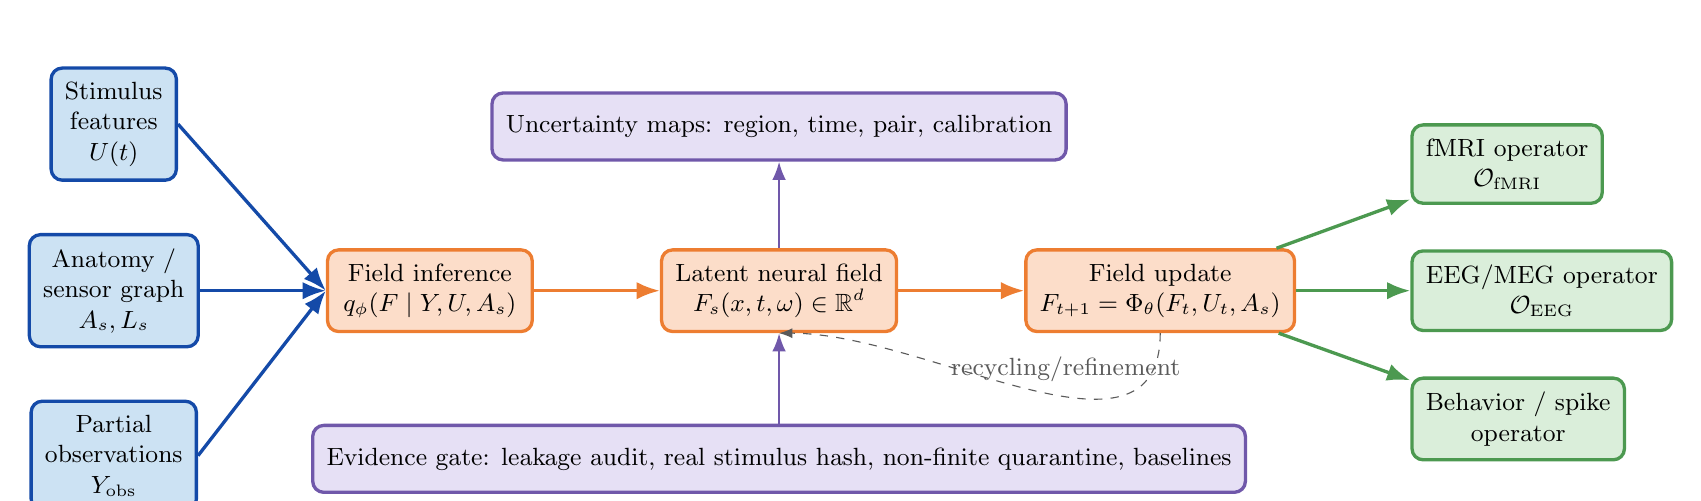
\begin{tikzpicture}[>=Latex, font=\small, node distance=1.2cm]
\tikzstyle{block}=[draw=nfcBlue, very thick, rounded corners, fill=nfcLightBlue, minimum height=1.0cm, align=center, inner sep=5pt]
\tikzstyle{op}=[draw=nfcOrange, very thick, rounded corners, fill=nfcLightOrange, minimum height=1.0cm, align=center, inner sep=5pt]
\tikzstyle{gate}=[draw=nfcGreen, very thick, rounded corners, fill=nfcLightGreen, minimum height=0.85cm, align=center, inner sep=5pt]
\tikzstyle{warn}=[draw=nfcPurple, very thick, rounded corners, fill=nfcLightPurple, minimum height=0.85cm, align=center, inner sep=5pt]

\node[block] (stim) {Stimulus\\features\\$U(t)$};
\node[block, below=0.65cm of stim] (anat) {Anatomy /\\sensor graph\\$A_s,L_s$};
\node[block, below=0.65cm of anat] (obs) {Partial\\observations\\$Y_{\rm obs}$};

\node[op, right=1.6cm of anat, minimum width=2.6cm] (infer) {Field inference\\$q_\phi(F\mid Y,U,A_s)$};
\node[op, right=1.6cm of infer, minimum width=2.6cm] (field) {Latent neural field\\$F_s(x,t,\omega)\in\mathbb{R}^d$};
\node[op, right=1.6cm of field, minimum width=2.6cm] (update) {Field update\\$F_{t+1}=\Phi_\theta(F_t,U_t,A_s)$};

\node[gate, above right=0.55cm and 1.45cm of update] (fmri) {fMRI operator\\$\mathcal{O}_{\rm fMRI}$};
\node[gate, right=1.45cm of update] (eeg) {EEG/MEG operator\\$\mathcal{O}_{\rm EEG}$};
\node[gate, below right=0.55cm and 1.45cm of update] (beh) {Behavior / spike\\operator};

\node[warn, below=1.15cm of field, minimum width=5.2cm] (evidence) {Evidence gate: leakage audit, real stimulus hash, non-finite quarantine, baselines};
\node[warn, above=1.1cm of field, minimum width=5.2cm] (unc) {Uncertainty maps: region, time, pair, calibration};

\draw[->, very thick, nfcBlue] (stim.east) -- (infer.west);
\draw[->, very thick, nfcBlue] (anat.east) -- (infer.west);
\draw[->, very thick, nfcBlue] (obs.east) -- (infer.west);
\draw[->, very thick, nfcOrange] (infer) -- (field);
\draw[->, very thick, nfcOrange] (field) -- (update);
\draw[->, very thick, nfcGreen] (update) -- (fmri);
\draw[->, very thick, nfcGreen] (update) -- (eeg);
\draw[->, very thick, nfcGreen] (update) -- (beh);
\draw[->, thick, nfcPurple] (evidence) -- (field);
\draw[->, thick, nfcPurple] (field) -- (unc);
\draw[->, dashed, nfcGray] (update.south) to[out=-90,in=0] (field.south);
\node[below=0.18cm of update, xshift=-1.2cm, text=nfcGray] {recycling/refinement};
\end{tikzpicture}%
}
\caption{\textbf{NeuroTwin NFC architecture schematic.} The central claim is not multimodal fusion. The model infers a latent neural field and compiles it into observations through modality-specific operators. Evidence gates and uncertainty maps are part of the scientific output, not decoration. All panels in later implementation figures should follow this style: tensor, operator, claim boundary.}
\end{figure}

\begin{figure}[p]
\centering
\resizebox{0.98\linewidth}{!}{%
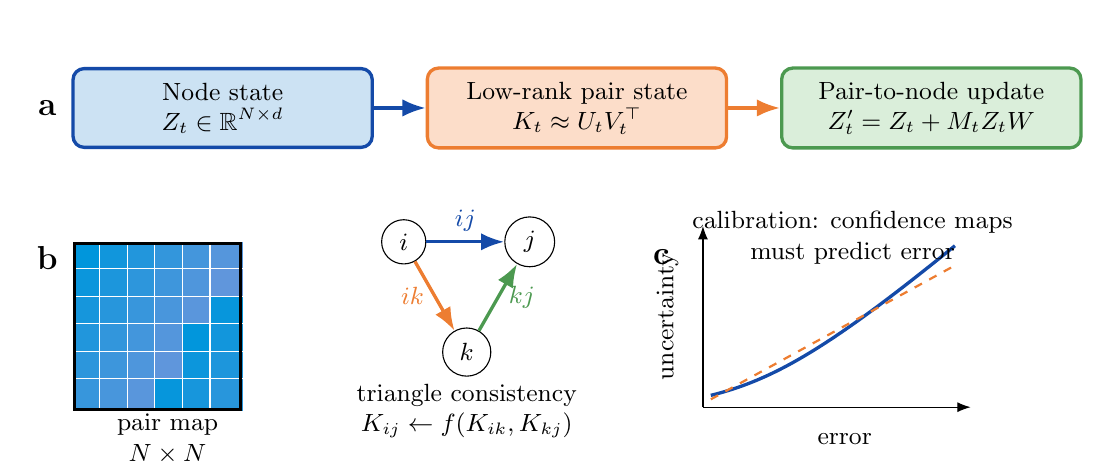
\begin{tikzpicture}[>=Latex, font=\small]
\tikzstyle{cell}=[draw=white, minimum width=0.42cm, minimum height=0.42cm]
\tikzstyle{box}=[draw=nfcBlue, very thick, rounded corners, fill=nfcLightBlue, align=center, inner sep=5pt]
\tikzstyle{orangebox}=[draw=nfcOrange, very thick, rounded corners, fill=nfcLightOrange, align=center, inner sep=5pt]
\tikzstyle{greenbox}=[draw=nfcGreen, very thick, rounded corners, fill=nfcLightGreen, align=center, inner sep=5pt]

\node at (-0.5,5.2) {\panel{a}};
\node[box, minimum width=3.8cm, minimum height=1cm] (nodes) at (1.7,5.2) {Node state\\$Z_t\in\mathbb{R}^{N\times d}$};
\node[orangebox, minimum width=3.8cm, minimum height=1cm] (pairs) at (6.2,5.2) {Low-rank pair state\\$K_t\approx U_tV_t^\top$};
\node[greenbox, minimum width=3.8cm, minimum height=1cm] (msg) at (10.7,5.2) {Pair-to-node update\\$Z'_t=Z_t+M_tZ_tW$};
\draw[->, very thick, nfcBlue] (nodes) -- (pairs);
\draw[->, very thick, nfcOrange] (pairs) -- (msg);

\node at (-0.5,3.3) {\panel{b}};
\foreach \i in {0,...,5}{\foreach \j in {0,...,5}{\pgfmathsetmacro\v{int(mod(17*\i+11*\j,100))}\definecolor{tmp}{RGB}{\v,150,220}\node[cell, fill=tmp] at (0.35*\i,3.3-0.35*\j) {};}}
\draw[very thick] (-0.18,3.48) rectangle (1.93,1.37);
\node[align=center] at (1.0,1.0) {pair map\\$N\times N$};
\node[draw, circle, fill=white] (i) at (4.0,3.5) {$i$};
\node[draw, circle, fill=white] (j) at (5.6,3.5) {$j$};
\node[draw, circle, fill=white] (k) at (4.8,2.1) {$k$};
\draw[->, very thick, nfcBlue] (i) -- node[above] {$ij$} (j);
\draw[->, very thick, nfcOrange] (i) -- node[left] {$ik$} (k);
\draw[->, very thick, nfcGreen] (k) -- node[right] {$kj$} (j);
\node[align=center] at (4.8,1.35) {triangle consistency\\$K_{ij}\leftarrow f(K_{ik},K_{kj})$};

\node at (7.3,3.3) {\panel{c}};
\draw[->] (7.8,1.4) -- (7.8,3.7);
\draw[->] (7.8,1.4) -- (11.2,1.4);
\node[rotate=90] at (7.35,2.55) {uncertainty};
\node at (9.6,1.0) {error};
\draw[nfcBlue, very thick] (7.9,1.55) .. controls (8.7,1.75) and (9.4,2.15) .. (11.0,3.45);
\draw[nfcOrange, thick, dashed] (7.9,1.5) -- (11.0,3.2);
\node[align=center] at (9.7,3.55) {calibration: confidence maps\\must predict error};
\end{tikzpicture}%
}
\caption{\textbf{Pair-state and confidence-map standard.} a, Low-rank pair state is a computationally feasible substitute for dense parcel-pair tensors. b, Triangle consistency mirrors the principle that pairwise relations must be mutually compatible; in NeuroTwin this is a brain-network relation, not protein geometry. c, Uncertainty maps are evaluated by calibration, not vibes.}
\end{figure}

\begin{figure}[p]
\centering
\resizebox{0.98\linewidth}{!}{%
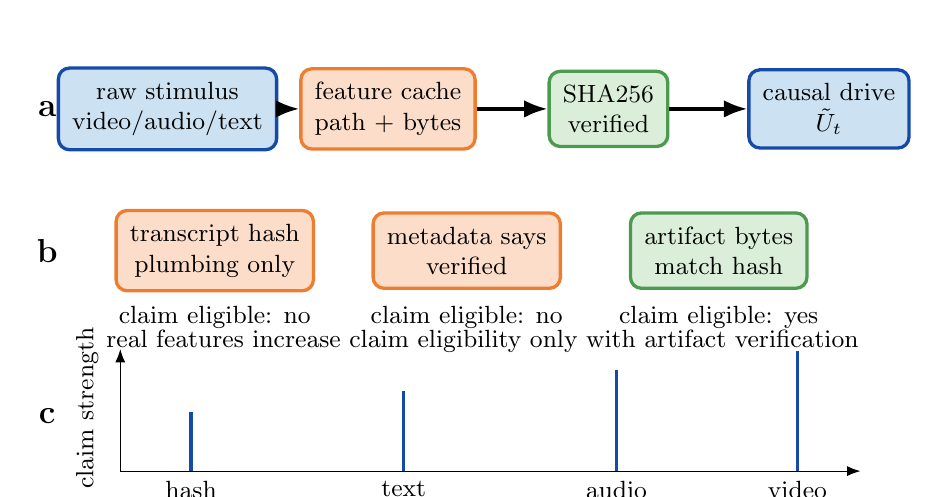
\begin{tikzpicture}[>=Latex, font=\small]
\tikzstyle{blk}=[draw=nfcBlue, very thick, rounded corners, fill=nfcLightBlue, align=center, minimum height=0.8cm, inner sep=5pt]
\tikzstyle{org}=[draw=nfcOrange, very thick, rounded corners, fill=nfcLightOrange, align=center, minimum height=0.8cm, inner sep=5pt]
\tikzstyle{grn}=[draw=nfcGreen, very thick, rounded corners, fill=nfcLightGreen, align=center, minimum height=0.8cm, inner sep=5pt]
\node at (-0.3,5.0) {\panel{a}};
\node[blk] (raw) at (1.2,5.0) {raw stimulus\\video/audio/text};
\node[org] (cache) at (4.0,5.0) {feature cache\\path + bytes};
\node[grn] (hash) at (6.8,5.0) {SHA256\\verified};
\node[blk] (drive) at (9.6,5.0) {causal drive\\$\tilde U_t$};
\draw[->, very thick] (raw) -- (cache);
\draw[->, very thick] (cache) -- (hash);
\draw[->, very thick] (hash) -- (drive);
\node at (-0.3,3.2) {\panel{b}};
\node[org] (no1) at (1.8,3.2) {transcript hash\\plumbing only};
\node[org] (no2) at (5.0,3.2) {metadata says\\verified};
\node[grn] (yes) at (8.2,3.2) {artifact bytes\\match hash};
\node[align=center] at (1.8,2.35) {claim eligible: no};
\node[align=center] at (5.0,2.35) {claim eligible: no};
\node[align=center] at (8.2,2.35) {claim eligible: yes};
\node at (-0.3,1.1) {\panel{c}};
\draw[->] (0.6,0.4) -- (0.6,1.95);
\draw[->] (0.6,0.4) -- (10.0,0.4);
\foreach \x/\lab in {1.5/hash,4.2/text,6.9/audio,9.2/video}{\draw[nfcBlue, very thick] (\x,0.4) -- (\x,1.0+0.2*\x/2); \node[below] at (\x,0.4) {\lab};}
\node[rotate=90] at (0.18,1.2) {claim strength};
\node at (5.2,2.05) {real features increase claim eligibility only with artifact verification};
\end{tikzpicture}%
}
\caption{\textbf{Stimulus evidence gate.} The model must not mistake synthetic or hash-only stimulus features for real perceptual encoders. Claim eligibility requires source artifact verification, not self-attested metadata or in-memory embedding hashes.}
\end{figure}



\section{Executive Thesis}

The central claim of this document is:
\begin{quote}
\textbf{Brain recordings should be modeled as an inverse problem over a latent neural field. Each modality is a lossy observation operator. Learning should infer the field and the operators jointly, with stability, uncertainty, and evidence constraints.}
\end{quote}

Current neural modeling pipelines often treat data as windows:
\begin{equation}
\text{EEG/fMRI/stimulus windows} \longrightarrow \text{model} \longrightarrow \text{prediction}.
\end{equation}
This is a useful engineering path, but not a revolutionary primitive. The proposed replacement is:
\begin{equation}
\text{partial observations} + \text{stimulus} + \text{anatomy}
\longrightarrow F_s(x,t,\omega)
\longrightarrow \Obs_m(F_s)
\longrightarrow Y_m.
\end{equation}
The latent object is not a token sequence in the usual sense. It is a hidden field over brain position, time, scale/frequency, and subject state:
\begin{equation}
F_s(x,t,\omega) \in \R^d.
\end{equation}
Observed modalities are measurements of this field:
\begin{equation}
Y_m = \Obs_m(F_s,A_s,U,\epsilon_m),
\end{equation}
where $m$ indexes modality, $A_s$ denotes subject anatomy, geometry, sensor layout, or connectome priors, $U$ is stimulus/task drive, and $\epsilon_m$ is modality-specific noise.

\subsection{The Primitive}

The primitive is:
\begin{quote}
\textbf{Many sensors, one field.}
\end{quote}

The Transformer primitive was attention:
\begin{equation}
\operatorname{Attention}(Q,K,V) = \softmax\left(\frac{QK^\top}{\sqrt{d}}\right)V.
\end{equation}
Mamba's primitive was selective state propagation:
\begin{equation}
h_{t+1} = A(x_t)h_t + B(x_t)x_t,
\end{equation}
where the state-space parameters depend on the input, allowing selective propagation or forgetting across long sequences \cite{mamba}. AlphaFold's primitive was relational geometry: model structure through pairwise constraints and confidence maps rather than independent residue predictions \cite{alphafold2,alphafold3}. NeuroTwin NFC's primitive is observation compilation:
\begin{equation}
\boxed{Y_m(t) = \Obs_m(F_s(x,t,\omega)).}
\end{equation}
The model does not fuse modalities. It compiles latent brain dynamics into modality-specific observations.

\section{Research Process and Design History}

This section records the auditable research process that produced the current architecture. It is intentionally high-level. It is not a hidden chain-of-thought transcript. It is a design log for keeping future code aligned with the research thesis.

\subsection{Phase 0: Brain-Inspired Starting Point}

The project began with interest in brain-inspired AI systems: sparse representations, online update, Hebbian-like learning, surprise gates, homeostasis, and concept graphs. These ideas were useful as inspiration, but they were too vague to support a publishable claim. The first design correction was:
\begin{quote}
Do not claim ``brain-like'' unless the mechanism is measurable, ablated, and validated under leakage-safe splits.
\end{quote}

\subsection{Phase 1: NeuroTwin as Neural Translation}

The first rigorous formulation was NeuroTwin as a neural translation system:
\begin{equation}
\text{EEG/fMRI/stimulus/behavior} \longrightarrow \text{shared latent state} \longrightarrow \text{forecast/reconstruct/translate}.
\end{equation}
This produced valuable infrastructure: event manifests, split manifests, leakage audits, baseline tables, multi-seed reporting, identity probes, model cards, and claim gates. However, the model architecture remained close to standard sequence modeling.

\subsection{Phase 2: TRIBE v2 and BrainVista Forced a Pivot}

TRIBE v2 reframed the stimulus-to-fMRI lane by scaling tri-modal video/audio/language encoding over more than 1,000 hours of fMRI across 720 subjects \cite{tribev2}. BrainVista reframed naturalistic fMRI as multimodal next-token prediction with causal stimulus-to-brain masking and network-wise tokenization \cite{brainvista}. These works made it unsafe to claim novelty from ``stimulus to fMRI'' alone. The design rule became:
\begin{quote}
TRIBE-style and BrainVista-style models are baselines or reference lanes, not the NeuroTwin claim.
\end{quote}

\subsection{Phase 3: Pair-Operator as Architecture Candidate}

Pair-Operator introduced explicit parcel/region pair states:
\begin{equation}
Z_t \in \R^{N\times d}, \qquad P_t \in \R^{N\times N\times r},
\end{equation}
with low-rank factorization to avoid $O(N^2)$ blowup. This was closer to AlphaFold-style relational modeling. But Pair-Operator was still a layer, not a paradigm. It answered:
\begin{quote}
How do parcels interact?
\end{quote}
It did not fully answer:
\begin{quote}
What are EEG, fMRI, MEG, spikes, and behavior actually observations of?
\end{quote}

\subsection{Phase 4: Neural Field Compiler}

The deeper architecture emerged by treating all brain recordings as observation operators over one latent neural field. Pair-Operator becomes a field-update submodule. EEG and fMRI are no longer modalities to fuse; they are measurement operators.

\subsection{Phase 5: Evidence Discipline}

The empirical process showed that simple baselines, especially ridge and autoregressive ridge, can beat current neural models on MOABB EEG. This is not failure; it is evidence. It implies that linear structure is strong and must be included rather than fought blindly. The architecture therefore includes Koopman-residual dynamics:
\begin{equation}
F_{t+1} = KF_t + R_\theta(F_t,U_t),
\end{equation}
where $K$ captures stable linear dynamics and $R_\theta$ captures nonlinear residual structure.

\section{Positioning Against Frontier Work}

\subsection{TRIBE v2}

TRIBE v2 is a tri-modal video/audio/language foundation model capable of predicting fMRI responses across naturalistic and experimental conditions, trained on more than 1,000 hours of fMRI across 720 subjects \cite{tribev2}. Its contribution is a scaled stimulus-to-fMRI encoding model and an in-silico neuroscience framework. NeuroTwin NFC should not claim first stimulus-to-brain modeling. Instead, it should claim field/operator factorization:
\begin{equation}
\text{stimulus} \longrightarrow F \longrightarrow \text{fMRI, EEG, behavior, etc.}
\end{equation}
TRIBE predicts a target modality. NFC infers a latent field and renders observations.

\subsection{BrainVista}

BrainVista treats naturalistic fMRI as multimodal next-token prediction, addressing timescale mismatch between high-frequency stimuli and hemodynamically filtered fMRI with stimulus-to-brain masking \cite{brainvista}. NeuroTwin NFC should borrow the principle of causal alignment:
\begin{equation}
\tilde{U}_t = \sum_{\ell=0}^L \alpha_\ell U_{t-\ell},
\end{equation}
without copying BrainVista's implementation or claiming exact reproduction.

\subsection{Brain-OF and BrainOmni}

Brain-OF proposes a unified fMRI/EEG/MEG foundation model with any-resolution sampling, DINT attention, Sparse Mixture of Experts, and masked temporal-frequency modeling \cite{brainof}. BrainOmni unifies EEG/MEG through a sensor-aware tokenizer encoding layout, orientation, and sensor type \cite{brainomni}. These works occupy the ``brain foundation model'' and ``modality unification'' space. NeuroTwin NFC should not claim first foundation model. It should claim a different factorization:
\begin{equation}
\text{modality} = \text{observation operator over shared field}.
\end{equation}

\subsection{AlphaFold and Pairwise Relational State}

AlphaFold's impact came from representing molecular structure through relational constraints, geometry, iterative refinement, and confidence maps \cite{alphafold2,alphafold3}. NeuroTwin NFC's analog is not protein geometry. It is brain-field relational state:
\begin{equation}
K_t(i,j) \approx U_i(t)V_j(t)^\top,
\end{equation}
with uncertainty maps over parcel pairs:
\begin{equation}
\operatorname{NPU}_{ij}(t)=\E\left[\left\|K_{ij}(t)-\hat{K}_{ij}(t)\right\|\right].
\end{equation}

\subsection{Mamba and Selective State Dynamics}

Mamba identifies the weakness of fixed subquadratic sequence models and makes state-space parameters input-dependent \cite{mamba}. NeuroTwin NFC should use selective state principles for temporal field updates:
\begin{equation}
F_{t+1}=A_\theta(U_t)F_t + B_\theta(U_t)U_t.
\end{equation}
This is especially important for fMRI and EEG because their time scales differ by orders of magnitude.

\subsection{DeepSeek-Style Sparse Experts}

DeepSeek-V3 demonstrates how sparse expert activation and latent attention can decouple parameter count from active compute \cite{deepseekv3}. NFC should use brain-structured experts rather than generic MoE:
\begin{equation}
F' = F + \sum_{e\in \operatorname{TopK}(g_\theta(F,U,m,A_s))} \pi_e E_e(F).
\end{equation}
Experts should correspond to brain or measurement structure: visual, auditory, language, default-mode, motor, hemodynamic, sensor-noise, uncertainty.

\section{Core Mathematical Formulation}

\subsection{Latent Field}

Let $\Omega$ be a cortical domain, atlas graph, or sensor/source space. The hidden field is
\begin{equation}
F_s:\Omega\times \mathbb{T}\times \Lambda \rightarrow \R^d,
\end{equation}
where $\mathbb{T}$ is time and $\Lambda$ is scale/frequency. A discretized version over $N$ parcels and $T$ time points is
\begin{equation}
Z \in \R^{B\times T\times N\times d}.
\end{equation}

\subsection{Generative Model}

The generative process is:
\begin{align}
F_0 &\sim p(F_0\mid A_s),\\
F_t &\sim p_\theta(F_t\mid F_{t-1},U_t,A_s),\\
Y_{m,t} &\sim p_\theta(Y_{m,t}\mid F_t,A_s).
\end{align}
Thus
\begin{equation}
p_\theta(F_{0:T},Y_{1:M}\mid U,A_s)=p(F_0)\prod_{t=1}^T p_\theta(F_t\mid F_{t-1},U_t,A_s)\prod_{m=1}^M p_\theta(Y_{m,t}\mid F_t,A_s).
\end{equation}

\subsection{Inference Model}

Given partial observations:
\begin{equation}
Y_{\mathrm{obs}} = \{Y_m: m\in \mathcal{M}_{\mathrm{obs}}\},
\end{equation}
we infer:
\begin{equation}
q_\phi(F_{0:T}\mid Y_{\mathrm{obs}},U,A_s).
\end{equation}
Cross-modal translation factors as:
\begin{equation}
\hat{Y}_b = \Obs_b\left(\Infer_a(Y_a,U,A_s)\right).
\end{equation}
Direct translation $T_{a\rightarrow b}(Y_a)$ is a baseline. NFC wins only if the factorized path beats direct translation:
\begin{equation}
\Obs_b\circ \Infer_a \succ T_{a\rightarrow b}.
\end{equation}

\section{Functional Analysis and Operator Learning}

Classical neural networks learn maps between finite-dimensional Euclidean spaces:
\begin{equation}
f_\theta:\R^n\rightarrow \R^m.
\end{equation}
But neural data are sampled fields. NFC should learn maps between function spaces:
\begin{equation}
\Operator:\mathcal{Y}_{\mathrm{partial}}\times \mathcal{U}\times \mathcal{A}\rightarrow \mathcal{F}.
\end{equation}
DeepONet is relevant because it uses a branch network for sampled input functions and a trunk network for output coordinates, supported by universal approximation theorems for nonlinear operators \cite{deeponet}. Fourier Neural Operator is relevant because it parameterizes integral kernels in Fourier space and learns solution operators for PDE families \cite{fno}. The key coding implication is:
\begin{quote}
Do not hard-code a single resolution/window shape as the mathematical object. Treat it as a discretization of an underlying field/operator.
\end{quote}

\subsection{Operator Form}

Let $a\in \mathcal{A}$ parameterize anatomy, subject geometry, or task context. Let $u\in\mathcal{U}$ be stimulus drive. The field solver is:
\begin{equation}
F = \mathcal{G}_\theta(y_{\mathrm{partial}},u,a).
\end{equation}
Observation rendering is:
\begin{equation}
\hat{y}_m = \Obs_{m,\theta}(F,a).
\end{equation}

\section{Functional Equations and Controlled Dynamics}

A field flow satisfies a semigroup property in the autonomous case:
\begin{equation}
\Phi_{\Delta_1+\Delta_2}=\Phi_{\Delta_2}\circ \Phi_{\Delta_1}.
\end{equation}
For stimulus-driven dynamics:
\begin{equation}
F(t+\Delta)=\Phi_{\theta,\Delta}\left(F(t),U_{[t-H,t]},A_s\right).
\end{equation}
For irregularly sampled observations, a controlled differential equation is natural:
\begin{equation}
dF_t = f_\theta(F_t)dt + g_\theta(F_t)dU_t.
\end{equation}
Neural CDEs provide a framework for partially observed irregular time series and can use memory-efficient adjoint backpropagation \cite{neuralcde}. The coding implication is:
\begin{quote}
Represent timestamps explicitly. Do not force all modalities onto one arbitrary grid if it introduces leakage, aliasing, or hemodynamic confusion.
\end{quote}

\section{Neural-Field Calculus}

A biologically shaped field equation is:
\begin{equation}
\tau \frac{\partial F(x,t)}{\partial t}
= -F(x,t)+\int_\Omega K_\theta(x,x',t)\sigma(F(x',t))dx' + B_\theta U(t)+\eta(x,t).
\end{equation}
Discretized over $N$ nodes:
\begin{equation}
Z_{t+1}=Z_t+\Delta t\left[-DZ_t+K_t\sigma(Z_t)+BU_t\right]+\xi_t.
\end{equation}
Here $K_t$ is dynamic coupling. Pair-Operator is a parameterization of $K_t$, not the whole theory.

\section{Graph Calculus and Anatomy Priors}

Let $G=(V,E,w)$ be a weighted graph over brain regions or sensors. The graph derivative along edge $(i,j)$ is:
\begin{equation}
\nabla_w F(i,j)=\sqrt{w_{ij}}(F_j-F_i).
\end{equation}
The graph Laplacian is:
\begin{equation}
L=D-W.
\end{equation}
Graph smoothness is:
\begin{equation}
R_{\mathrm{graph}}(F)=\sum_{(i,j)\in E}w_{ij}\|F_i-F_j\|^2=\tr(F^\top L F).
\end{equation}
The latent field is not free-floating. It lives on a brain graph. The field update may include:
\begin{equation}
F_{t+1}=F_t+\Delta t\left[-\alpha L_sF_t+\mathcal{N}_\theta(F_t,U_t)\right].
\end{equation}

\section{Linear Algebra: Low-Rank Relational State}

A full pair kernel $K_t\in\R^{N\times N}$ is expensive. Use low-rank factorization:
\begin{equation}
K_t\approx U_tV_t^\top,
\qquad U_t,V_t\in\R^{N\times r}, \quad r\ll N.
\end{equation}
The induced message matrix is:
\begin{equation}
M_t = \softmax\left(\frac{U_tV_t^\top}{\sqrt{r}} + S\right),
\end{equation}
where $S$ is an anatomical or structural prior. Node update:
\begin{equation}
Z'_t = Z_t + M_t Z_t W.
\end{equation}

\subsection{Approximation Guarantee}

By truncated singular value decomposition, if $K_t$ has singular values $\sigma_1\geq\sigma_2\geq\cdots$, then the best rank-$r$ approximation $K_t^{(r)}$ satisfies:
\begin{equation}
\|K_t-K_t^{(r)}\|_F^2=\sum_{j>r}\sigma_j^2.
\end{equation}
Thus low-rank pair state is justified if brain network interactions are compressible.

\section{Observation Operators}

\subsection{fMRI Observation Operator}

fMRI measures hemodynamically filtered neural activity. Let $h_{\mathrm{HRF}}$ be an HRF kernel:
\begin{equation}
(H_{\mathrm{HRF}}a)(t)=\int_0^\infty h(\tau)a(t-\tau)d\tau.
\end{equation}
Then:
\begin{equation}
Y_{\mathrm{fMRI}}(p,t)=R_pH_{\mathrm{HRF}}g_\theta(F(\cdot,t))+\epsilon.
\end{equation}
A causal finite approximation is:
\begin{equation}
\tilde{U}_t=\sum_{\ell=0}^{L}\alpha_\ell U_{t-\ell}.
\end{equation}
No future stimulus terms may appear in $\tilde{U}_t$ for a claim-eligible causal prediction.

\subsection{EEG/MEG Observation Operator}

EEG/MEG are electromagnetic projections of neural currents:
\begin{align}
Y_{\mathrm{EEG}}(t)&=L_sJ_\theta(F_t)+\epsilon_{\mathrm{EEG}},\\
Y_{\mathrm{MEG}}(t)&=M_sJ_\theta(F_t)+\epsilon_{\mathrm{MEG}}.
\end{align}
The important point is that EEG and MEG are not independent data worlds. They are different observation operators of neural current fields.

\subsection{Spike and Calcium Observation Operators}

For spikes:
\begin{equation}
Y_{n,t}\sim \Poisson\left(\Delta t\cdot \operatorname{softplus}(w_n^\top F(x_n,t))\right).
\end{equation}
For calcium:
\begin{equation}
C_{n,t}=(k_{\mathrm{Ca}}*r_n)(t)+\epsilon.
\end{equation}
These are deferred implementation targets, not v0 requirements.

\subsection{Behavior Observation Operator}

For discrete behavior:
\begin{equation}
p(a_t\mid F_t,U_t)=\softmax\left(C\operatorname{pool}(F_t)+DU_t\right).
\end{equation}

\section{Variational Inference and Missing Modalities}

NFC is naturally trained with missing observations. The ELBO is:
\begin{equation}
\mathcal{L}_{\mathrm{ELBO}}
=\E_{q_\phi}\left[\sum_{m,t}\log p_\theta(Y_{m,t}\mid F_t,A_s)\right]
-\beta\KL\left(q_\phi(F\mid Y,U,A_s)\|p_\theta(F\mid U,A_s)\right).
\end{equation}
This makes cross-modal learning possible even when not all modalities are observed for all samples.

\subsection{Masked Observation Training}

Given observed set $\mathcal{M}_{\mathrm{obs}}$ and hidden set $\mathcal{M}_{\mathrm{mask}}$:
\begin{equation}
F\sim q_\phi(F\mid \{Y_m:m\in\mathcal{M}_{\mathrm{obs}}\},U,A_s),
\end{equation}
then render:
\begin{equation}
\hat{Y}_b=\Obs_b(F,A_s), \quad b\in\mathcal{M}_{\mathrm{mask}}.
\end{equation}

\section{Identifiability and Gauge Symmetry}

Latent fields are not identifiable without constraints. If:
\begin{equation}
F'=AF,
\end{equation}
and
\begin{equation}
\Obs'_m=\Obs_mA^{-1},
\end{equation}
then:
\begin{equation}
\Obs'_m(F')=\Obs_m(F).
\end{equation}
The observations cannot distinguish $F$ from $F'$. This is a gauge ambiguity.

\subsection{Gauge-Fixing Constraints}

We impose:
\begin{align}
R_{\mathrm{graph}}(F)&=\tr(F^\top LF),\\
R_{\mathrm{time}}(F)&=\sum_t\|F_{t+1}-F_t\|^2,\\
R_{\mathrm{band}}(F)&=\sum_\omega \gamma_\omega\|\hat{F}(\omega)\|^2.
\end{align}
Subject adapters are restricted:
\begin{equation}
A_s=I+U_sV_s^\top,
\end{equation}
so a subject cannot learn an unconstrained private coordinate system.

\section{Stability Theory}

For continuous dynamics:
\begin{equation}
\frac{dF}{dt}=f_\theta(F,U,t).
\end{equation}
The local Jacobian is:
\begin{equation}
J_t=\frac{\partial f_\theta}{\partial F}.
\end{equation}
Local stability requires:
\begin{equation}
\Re(\lambda_i(J_t))<0.
\end{equation}
For discrete linearized dynamics:
\begin{equation}
F_{t+1}=AF_t,
\end{equation}
stability requires:
\begin{equation}
\rho(A)<1,
\end{equation}
where $\rho$ is spectral radius. A practical regularizer is:
\begin{equation}
R_{\mathrm{stab}}=\max(0,\rho(A)-1)^2.
\end{equation}
This connects directly to coding requirements: non-finite loss detection, gradient clipping, best finite checkpoint selection, task quarantine, and no hidden NaNs.

\section{Uncertainty and Calibration}

Each observation operator should output a predictive distribution:
\begin{equation}
Y_{m,t}\sim\N(\mu_{m,t},\Sigma_{m,t}).
\end{equation}
For diagonal variance:
\begin{equation}
\loss_{\mathrm{NLL}}=\sum_{m,t,i}\frac{(y_{m,t,i}-\mu_{m,t,i})^2}{2\sigma_{m,t,i}^2}+\frac{1}{2}\log\sigma_{m,t,i}^2.
\end{equation}
Calibration means:
\begin{equation}
\mathbb{P}\left(Y\in C_\alpha(X)\right)\approx 1-\alpha.
\end{equation}
The model should report:
\begin{itemize}
\item error--uncertainty correlation,
\item expected calibration error,
\item coverage at 50\%, 80\%, and 90\%,
\item regionwise uncertainty maps,
\item pairwise uncertainty maps.
\end{itemize}

\section{Information Theory}

The latent field should keep shared neural information and discard sensor-specific noise:
\begin{equation}
\max_F \sum_m \MI(F;Y_m)-\lambda \MI(F;N_m).
\end{equation}
For cross-modal consistency:
\begin{equation}
\MI(F_{\mathrm{EEG}};F_{\mathrm{fMRI}})
\end{equation}
should be high for shared neural content. Contrastive objectives may be used:
\begin{equation}
\loss_{\mathrm{InfoNCE}}=-\log\frac{\exp(\operatorname{sim}(z_a,z_b)/\tau)}{\sum_{b'}\exp(\operatorname{sim}(z_a,z_{b'})/\tau)}.
\end{equation}
However, contrastive construction is dangerous under leakage. Negatives/positives must not share subject or stimulus segment when split policy forbids it.

\section{Koopman-Residual Dynamics}

If ridge beats deep models, the correct response is not to ignore ridge. Include linear dynamics explicitly:
\begin{equation}
F_{t+1}=KF_t+R_\theta(F_t,U_t).
\end{equation}
Koopman theory represents nonlinear dynamics as linear evolution over observables:
\begin{equation}
g(F_{t+1})=\mathcal{K}g(F_t).
\end{equation}
Deep Koopman networks learn dictionaries for these observables \cite{deepkoopman}. The NeuroTwin loss should include:
\begin{equation}
\loss=\loss_{\mathrm{pred}}+\lambda_R\|R_\theta\|^2+\lambda_K\max(0,\rho(K)-1)^2.
\end{equation}
Interpretation:
\begin{quote}
Let linear dynamics win when they are right. Make neural modeling explain only what linear structure cannot.
\end{quote}

\section{Riemannian Geometry for EEG}

EEG covariance:
\begin{equation}
C=\frac{1}{T}XX^\top
\end{equation}
lives on the symmetric positive definite manifold:
\begin{equation}
C\in\mathrm{SPD}(n).
\end{equation}
Riemannian EEG methods are strong because covariance geometry is not Euclidean \cite{riemannian}. A possible EEG observation head outputs covariance:
\begin{equation}
\hat{C}_{\mathrm{EEG}}=LL^\top+\epsilon I.
\end{equation}
Affine-invariant Riemannian distance:
\begin{equation}
d_{\mathrm{AIRM}}(C_1,C_2)=\left\|\log(C_1^{-1/2}C_2C_1^{-1/2})\right\|_F.
\end{equation}
This is useful for MOABB-like tasks and prevents the model from treating covariance objects as flat Euclidean vectors.

\section{Sampling, Lattices, and Number-Theoretic Nuance}

Each modality samples time on a lattice:
\begin{equation}
\mathcal{T}_m=\{k\Delta_m:k\in\mathbb{Z}\}.
\end{equation}
Examples:
\begin{itemize}
\item fMRI: slow TR lattice,
\item EEG: hundreds of Hz,
\item video: 24/30 fps,
\item audio: kHz,
\item text: irregular events.
\end{itemize}
If two sampling intervals have rational ratio:
\begin{equation}
\frac{\Delta_a}{\Delta_b}=\frac{p}{q},
\end{equation}
then exact alignment recurs every least common multiple of the integer grids. If timestamps drift or ratios are effectively irrational, alignment is not periodic.

Fourier positional features:
\begin{equation}
\phi(t)=\left[\sin(2\pi kt/T),\cos(2\pi kt/T)\right]_{k=1}^K.
\end{equation}
Graph spectral features:
\begin{equation}
Lv_k=\lambda_kv_k.
\end{equation}
For stress tests, use coprime window/stride pairs:
\begin{equation}
\gcd(w,s)=1,
\end{equation}
to avoid accidental periodic alignment and test aliasing/leakage.

\section{Computer-Science Complexity}

For $B$ batches, $T$ timepoints, $N$ nodes, latent dimension $d$, pair rank $r$:
\begin{align}
\text{node memory} &: O(BTNd),\\
\text{full pair memory} &: O(BTN^2r),\\
\text{low-rank pair memory} &: O(BTNr).
\end{align}
Temporal Transformer cost is:
\begin{equation}
O(T^2d),
\end{equation}
whereas SSM/Mamba-like temporal backbones target:
\begin{equation}
O(Td^2) \quad \text{or} \quad O(Td)
\end{equation}
depending on implementation. The desired complexity target is:
\begin{equation}
O(BTNr + BTNd^2 + BTd_{\mathrm{stim}}d),
\end{equation}
not:
\begin{equation}
O(BTN^2d + BT^2d).
\end{equation}
This makes the model realistic for 1,000 fMRI parcels and 6 A100 GPUs.

\section{Sparse Expert Computation}

Structured experts:
\begin{itemize}
\item visual-network expert,
\item auditory-network expert,
\item language-network expert,
\item default-mode expert,
\item motor expert,
\item hemodynamic expert,
\item EEG-sensor expert,
\item uncertainty expert.
\end{itemize}
Routing:
\begin{equation}
r=\operatorname{TopK}(g_\theta(F_t,U_t,m,A_s)).
\end{equation}
Expert update:
\begin{equation}
F'=F+\sum_{e\in r}\pi_eE_e(F).
\end{equation}
Load-balancing regularizer:
\begin{equation}
\loss_{\mathrm{load}}=\sum_e\left(\frac{n_e}{N_{\mathrm{tokens}}}-\frac{1}{E}\right)^2.
\end{equation}
Entropy regularizer:
\begin{equation}
\loss_{\mathrm{entropy}}=-\sum_e\pi_e\log\pi_e.
\end{equation}

\section{Commutative Diagram and API Discipline}

Modalities are objects $\mathcal{Y}_m$. The latent field space is $\mathcal{F}$. Inference maps:
\begin{equation}
\Infer_m:\mathcal{Y}_m\rightarrow\mathcal{F}.
\end{equation}
Observation maps:
\begin{equation}
\Obs_m:\mathcal{F}\rightarrow\mathcal{Y}_m.
\end{equation}
Cross-modal maps factor through the field:
\begin{equation}
T_{a\rightarrow b}=\Obs_b\circ \Infer_a.
\end{equation}
Direct $T_{a\rightarrow b}$ is a baseline, not the architecture.

\begin{center}
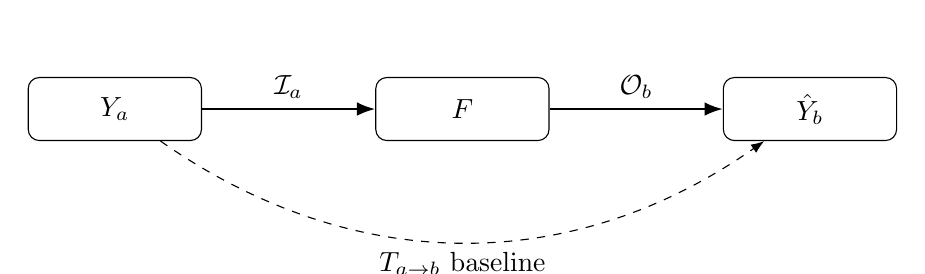
\begin{tikzpicture}[node distance=2.2cm,>=Latex]
\node (Ya) [draw, rounded corners, minimum width=2.2cm, minimum height=0.8cm] {$Y_a$};
\node (F) [draw, rounded corners, right=of Ya, minimum width=2.2cm, minimum height=0.8cm] {$F$};
\node (Yb) [draw, rounded corners, right=of F, minimum width=2.2cm, minimum height=0.8cm] {$\hat{Y}_b$};
\draw[->, thick] (Ya) -- node[above] {$\Infer_a$} (F);
\draw[->, thick] (F) -- node[above] {$\Obs_b$} (Yb);
\draw[->, dashed, bend right=35] (Ya) to node[below] {$T_{a\to b}$ baseline} (Yb);
\end{tikzpicture}
\end{center}

\section{Loss Hierarchy}

\subsection{Observation Reconstruction}
\begin{equation}
\loss_{\mathrm{rec}}=\sum_m\|Y_m-\hat{Y}_m\|^2.
\end{equation}

\subsection{Latent Dynamics}
Synthetic only, where true field is known:
\begin{equation}
\loss_{\mathrm{dyn}}=\|F_{t+1}-\Phi(F_t,U_t)\|^2.
\end{equation}

\subsection{Cycle Consistency}
\begin{equation}
\loss_{\mathrm{cycle}}=\|Y_a-\Obs_a(\Infer_b(Y_b))\|.
\end{equation}

\subsection{Uncertainty Calibration}
\begin{equation}
\loss_{\mathrm{nll}}=\frac{(y-\mu)^2}{2\sigma^2}+\frac{1}{2}\log\sigma^2.
\end{equation}

\subsection{Stability}
\begin{equation}
\loss_{\mathrm{stab}}=\max(0,\rho(K)-1)^2.
\end{equation}

\subsection{Evidence Gates}
Evidence gates are not differentiable losses. They are audit constraints:
\begin{lstlisting}
if leakage_audit_fails:
    scientific_claim_allowed = false
if real_stimulus_hash_fails:
    stimulus_claim_allowed = false
if required_task_nan:
    model_claim_allowed = false
if baseline_table_empty:
    model_superiority_claim_allowed = false
\end{lstlisting}

\section{Propositions for the Paper}

\subsection{Proposition 1: Direct Translation as a Special Case}
If $\Infer_a$ and $\Obs_b$ are sufficiently expressive, then $\Obs_b\circ\Infer_a$ can approximate any measurable direct map $T_{a\rightarrow b}$. Thus direct translation is a special case of field-mediated translation.

\subsection{Proposition 2: Latent Fields Improve Sample Efficiency Under Shared Generative Structure}
If multiple modalities are generated by conditionally independent observation operators over a shared low-dimensional latent field, then learning the shared field can reduce the effective sample complexity relative to separately learning pairwise translations. This is not an unconditional theorem for all data; it is an assumption to validate in synthetic field recovery.

\subsection{Proposition 3: Low-Rank Pair State Is Optimal Under Compressible Coupling}
For a dynamic coupling matrix $K_t$, the best rank-$r$ approximation error in Frobenius norm is the tail singular energy:
\begin{equation}
\min_{\rank(\tilde{K})\le r}\|K_t-\tilde{K}\|_F^2=\sum_{j>r}\sigma_j^2.
\end{equation}
Thus low-rank pair state is justified when effective brain coupling is compressible.

\subsection{Proposition 4: Ridge Winning Is Diagnostic}
If ridge or autoregressive ridge outperforms a neural model, either the task is dominated by linear structure, the neural model is under-optimized, or the architecture lacks the correct inductive bias. NFC should include linear/Koopman components rather than pretend nonlinearity is always superior.

\section{Architecture Specification}

\subsection{NeuroEventTokenizer}
Inputs:
\begin{itemize}
\item subject/session/site IDs,
\item modality,
\item time range,
\item sampling rate,
\item parcel/sensor/unit ID,
\item geometry/anatomy metadata,
\item stimulus ID/segment ID,
\item split ID,
\item source/preprocessing hashes,
\item evidence status.
\end{itemize}
Output token:
\begin{equation}
e_i=E_{\mathrm{mod}}+E_{\mathrm{time}}+E_{\mathrm{region}}+E_{\mathrm{subject}}+E_{\mathrm{safe-context}}.
\end{equation}
Evidence metadata is for gates/reports. It must not silently become predictive input if it leaks targets.

\subsection{LatentNeuralField}
Maintains:
\begin{equation}
F\in\R^{B\times T\times N\times d}.
\end{equation}

\subsection{FieldUpdateOperator}
\begin{equation}
F_{t+1}=F_t+\Delta_\theta(F_t,U_t,A_s,\Delta t).
\end{equation}
Backends:
\begin{itemize}
\item GRU/SSM fallback,
\item optional Mamba if cleanly installed,
\item graph/low-rank pair operator,
\item Koopman-residual component.
\end{itemize}

\subsection{Observation Operators}
\begin{itemize}
\item FMRIObservationOperator,
\item EEGObservationOperator,
\item BehaviorObservationOperator,
\item future SpikeObservationOperator,
\item future CalciumObservationOperator.
\end{itemize}

\subsection{Uncertainty Head}
Outputs:
\begin{itemize}
\item per-region uncertainty,
\item per-time uncertainty,
\item pairwise uncertainty,
\item calibration artifacts.
\end{itemize}

\section{Experiment Suite}

\subsection{Experiment A: Synthetic Field Recovery}
Generate latent field:
\begin{equation}
F_{t+1}=AF_t+K\sigma(F_t)+BU_t+\eta_t.
\end{equation}
Render:
\begin{align}
Y_{\mathrm{fMRI}}&=H_{\mathrm{HRF}}RF+\epsilon,\\
Y_{\mathrm{EEG}}&=LF+\epsilon.
\end{align}
Tasks:
\begin{itemize}
\item recover hidden $F$,
\item fMRI $\rightarrow$ EEG,
\item EEG $\rightarrow$ fMRI,
\item stimulus $\rightarrow$ fMRI,
\item masked reconstruction.
\end{itemize}
This is the first architecture claim. Do not skip it.

\subsection{Experiment B: Algonauts/CNeuroMod fMRI}
Use real stimulus features only. Compare:
\begin{itemize}
\item ridge,
\item autoregressive ridge,
\item BrainVista-style local approximation,
\item TRIBE-style clean-room approximation,
\item current NeuroTwin,
\item Pair-Operator,
\item NFC.
\end{itemize}
Tasks:
\begin{itemize}
\item future fMRI,
\item stimulus-to-fMRI,
\item masked parcels,
\item uncertainty calibration.
\end{itemize}

\subsection{Experiment C: MOABB EEG}
Use MOABB as reproducibility and field-observation sanity, not the main model battlefield. Tasks:
\begin{itemize}
\item future EEG,
\item masked EEG,
\item classification leakage demo,
\item identity probe,
\item EEG model card.
\end{itemize}

\section{Track A and Track B}

\subsection{Track A: Reproducibility Paper}
Claim:
\begin{quote}
NeuroTwin operationalizes EEG/neural-ML reproducibility through executable split manifests, leakage audits, identity probes, model cards, baselines, and claim gates.
\end{quote}
This track can succeed even when NeuroTwin loses to ridge.

\subsection{Track B: Model Paper}
Claim:
\begin{quote}
NeuroTwin NFC improves latent-field recovery and/or naturalistic brain prediction by factorizing neural data into shared field inference plus modality-specific observation operators.
\end{quote}
This track requires evidence that NFC beats direct baselines on synthetic field recovery and at least one real fMRI/stimulus task.

\section{Implementation Guardrails}

\subsection{Claim Hygiene}
\begin{itemize}
\item No clinical claims.
\item No SOTA claims.
\item No first-brain-foundation-model claims.
\item No exact TRIBE/BrainVista claims unless exact code/protocol/data are used.
\item No stimulus-to-fMRI claim from transcript hashes or synthetic features.
\item No model-superiority claim if ridge wins.
\end{itemize}

\subsection{Evidence Gates}
\begin{itemize}
\item Leakage audit must pass.
\item Baseline table must be nonempty.
\item Multi-seed evidence required for paper mode.
\item Confidence intervals required.
\item Quarantined required task disables claim.
\item Reports must be read-only.
\item Evidence finalization must be explicit.
\end{itemize}

\subsection{Stimulus Evidence}
Claim-eligible stimulus features require:
\begin{itemize}
\item source path or manifest URI,
\item modality list,
\item feature hash,
\item real or precomputed status,
\item hash verification from source artifact bytes.
\end{itemize}
Hashing an in-memory embedding is diagnostic only.

\section{Coding Roadmap}

\subsection{Milestone 1: NFC v0 Synthetic}
Build:
\begin{itemize}
\item LatentNeuralField,
\item FieldUpdateOperator,
\item FMRIObservationOperator,
\item EEGObservationOperator,
\item synthetic latent-field generator,
\item uncertainty head,
\item synthetic ablation suite.
\end{itemize}
Pass condition:
\begin{quote}
NFC full beats direct baseline on at least one synthetic latent-field recovery task. If it does not, report failure.
\end{quote}

\subsection{Milestone 2: Algonauts fMRI Debug}
Run one-A100 debug only after real stimulus features are verified. Check:
\begin{itemize}
\item no NaNs,
\item baseline table nonempty,
\item stimulus claim eligibility correct,
\item pair/field ablation outputs written,
\item uncertainty calibration artifact written.
\end{itemize}

\subsection{Milestone 3: Six-A100 Full Run}
Only after one-A100 debug passes. Compare against ridge, autoregressive ridge, BrainVista-style, TRIBE-style, current NeuroTwin, Pair-Operator, and NFC.

\subsection{Milestone 4: Paper Draft}
Write Track B paper only if NFC demonstrates an architecture win. Otherwise, write Track A first and keep NFC as ongoing research.

\section{Research Process Section for Future Paper}

This project intentionally evolved through several discarded hypotheses:
\begin{enumerate}
\item \textbf{Brain-inspired symbolic/plasticity modeling}: useful inspiration, insufficiently measurable.
\item \textbf{Generic multimodal NeuroTwin}: useful infrastructure, too close to Brain-OF/BrainOmni and too broad.
\item \textbf{Stimulus-to-fMRI direct modeling}: already occupied by TRIBE v2 and BrainVista.
\item \textbf{Pair-Operator}: useful relational module, but not a complete paradigm.
\item \textbf{Neural Field Compiler}: final current thesis: model hidden brain field plus observation operators.
\end{enumerate}
The guiding failures were just as important as wins. Ridge beating NeuroTwin forced a Koopman-residual design. NaN reconstruction forced non-finite quarantine and stability penalties. Hash-only stimulus features forced stimulus evidence gates. Leakage literature forced split manifests and claim gates.

\section{Kill Criteria}

Stop or downgrade Track B if:
\begin{itemize}
\item NFC cannot beat direct baselines on synthetic latent-field recovery.
\item NFC cannot beat Pair-Operator/no-field ablations.
\item Algonauts real-stimulus runs remain below ridge/BrainVista-style baselines.
\item uncertainty maps do not correlate with error.
\item real stimulus features cannot be verified.
\item NaN/quarantined tasks recur in required tasks.
\end{itemize}

\section{What Would Make This a High-Citation Paper}

Best-case contribution:
\begin{quote}
A strong demonstration that latent neural fields plus structured observation operators improve cross-modal and naturalistic brain prediction beyond direct baselines.
\end{quote}
Good-case contribution:
\begin{quote}
A rigorous mathematical framework unifying fMRI, EEG, and stimulus modeling as observation operators over a latent field, with executable evidence gates.
\end{quote}
Safe-case contribution:
\begin{quote}
A reproducibility infrastructure paper with synthetic proof-of-concept and strong leakage demos.
\end{quote}

\section{Conclusion}

NeuroTwin NFC is not ``bigger NeuroTwin.'' It is a different object. The deepest thesis is:
\begin{quote}
Brain data should be modeled as a latent field inverse problem. Each recording modality is a lossy observation operator. Learning should infer the field, evolve it through time, and compile it into observations under evidence-gated constraints.
\end{quote}
This is the architecture direction. If it works on synthetic latent-field recovery and then on Algonauts fMRI with real stimulus features, it becomes a serious model paper. If it does not, the project still has a strong reproducibility-track paper.

\appendix
\section{Minimal Codex Prompt for NFC v0}

\begin{lstlisting}
Implement NeuroTwin NFC v0.

Do not broaden modalities.
Do not train large models.
Do not run A100.

Build:
1. LatentNeuralField module
2. FieldUpdateOperator
3. FMRIObservationOperator
4. EEGObservationOperator
5. synthetic latent-field generator
6. NFC losses
7. uncertainty maps
8. evidence gate compatibility
9. tests and configs

Prove locally:
- latent field can render fMRI/EEG synthetic observations
- direct baselines and NFC can be compared
- NFC full beats direct baseline on at least one synthetic field recovery task
- if not, report failure

Run:
PYTHONPATH=src python3 -m unittest discover -s tests -v
PYTHONPATH=src python3 -m neurotwin.cli doctor
bash scripts/run_smoke.sh /tmp/neurotwin_nfc_smoke
git diff --check
graphify update .
\end{lstlisting}


\section{Coding Constitution for Preventing Research Drift}

The following rules are meant to be read by both humans and coding agents before each implementation sprint.

\subsection{Non-Negotiable Conceptual Rules}
\begin{enumerate}
\item NFC is a field-and-observation-operator model. Any implementation that becomes a direct multimodal fusion head is off-mission.
\item Pair-Operator is a submodule inside the FieldUpdateOperator. It is not the whole architecture.
\item Real stimulus claims require artifact-byte hash verification. Transcript hashes and synthetic embeddings are plumbing only.
\item Reports must be read-only. Finalization commands may write evidence sidecars; model-card rendering may not rewrite run evidence.
\item Linear baselines are not enemies. Ridge winning is evidence about the data-generating process.
\item NaNs are failures, not missing values. Quarantine must be visible and claim-blocking.
\item The model paper only exists if field/operator factorization beats direct baselines under leakage-gated evaluation on at least one real task.
\end{enumerate}

\subsection{Implementation Minimalism}
The first implementation should contain only the following real components:
\begin{enumerate}
\item latent field state tensor $F_{t}\in\R^{N\times d}$;
\item a field update operator with optional low-rank pair state;
\item fMRI observation operator with causal HRF/lag adapter;
\item EEG observation operator for synthetic and MOABB sanity tests;
\item synthetic latent-field generator;
\item uncertainty head;
\item evidence gate compatibility;
\item ablation configs.
\end{enumerate}
Do not add MEG, calcium, CT, spikes, or clinical outputs until the synthetic and fMRI core is proven.

\subsection{Ablation Law}
Every new mechanism must have a death test:
\begin{equation}
\Delta_{\mathrm{module}} = \mathrm{Metric}(\mathrm{full}) - \mathrm{Metric}(\mathrm{without\ module}).
\end{equation}
For lower-is-better metrics like MSE, define:
\begin{equation}
\Delta^{\mathrm{MSE}}_{\mathrm{module}} = \mathrm{MSE}(\mathrm{without}) - \mathrm{MSE}(\mathrm{full}).
\end{equation}
The module survives only if $\Delta$ is positive under the appropriate metric, across seeds, under the claim gate.

\section{Figure Roadmap for the Eventual Paper}

\begin{longtable}{p{0.16\linewidth}p{0.34\linewidth}p{0.40\linewidth}}
\toprule
Figure & AlphaFold-style role & NeuroTwin NFC content \\
\midrule
Fig. 1 & Architecture overview + information flow & Neural Field Compiler diagram with field, operators, evidence gate, uncertainty maps \\
Fig. 2 & Confidence validation & Region/time/pair uncertainty versus empirical error, calibration curves \\
Fig. 3 & Architecture details & Low-rank pair state, graph triangle consistency, field update operator \\
Fig. 4 & Ablations & Remove observation operators, pair state, HRF adapter, uncertainty head, subject adapter \\
Fig. 5 & Benchmark result & fMRI forecasting/stimulus response versus ridge, BrainVista-style, TRIBE-style clean-room, current NeuroTwin \\
Fig. 6 & Reproducibility gate & Leakage audit, identity probe, model card, claim gate, non-finite quarantine \\
\bottomrule
\end{longtable}

\section{Research Process: Final Decision Tree}

\subsection{If Synthetic NFC Fails}
If NFC does not beat direct baselines on synthetic latent-field recovery, do not run A100. The architecture is not yet coherent.

\subsection{If Synthetic NFC Passes but fMRI Fails}
Write Track A first: NeuroTwin as executable leakage audits and model gates. Keep NFC as future work.

\subsection{If fMRI NFC Beats Direct Baselines}
Proceed to model paper. The key claim becomes:
\begin{quote}
Field-mediated prediction improves naturalistic fMRI modeling over direct prediction under leakage-gated evaluation.
\end{quote}

\subsection{If NFC Beats Current NeuroTwin but Not Ridge}
Report an architecture improvement but not frontier performance. Analyze where ridge wins: parcel, network, subject, stimulus family, lag, signal-to-noise region.

\subsection{If NFC Beats Ridge or BrainVista-Style Baseline}
This is the real model-paper signal. Lock the split, rerun seeds, and prepare professor-facing technical summary.


\section{Reference Table for Prior Art}

\begin{longtable}{p{0.18\linewidth}p{0.36\linewidth}p{0.36\linewidth}}
\toprule
Work & Key contribution & NeuroTwin NFC lesson \\
\midrule
Transformer & Attention over tokens & A primitive matters more than size \\
Mamba & Selective state-space dynamics & Use selective long-time field updates \\
DeepONet/FNO & Operator learning between function spaces & Brain data are fields, not arrays \\
Neural CDE & Continuous-time irregular observation modeling & Do not force all modalities onto one grid \\
AlphaFold & Pairwise relational geometry and confidence & Use pair uncertainty for brain graphs \\
TRIBE v2 & Tri-modal stimulus-to-fMRI at scale & Do not claim first stimulus-to-fMRI \\
BrainVista & Causal fMRI next-token/stimulus masking & Include HRF/lag-aware causal stimulus adapter \\
Brain-OF & fMRI/EEG/MEG foundation model & Avoid generic foundation-model claims \\
BrainOmni & Sensor-aware EEG/MEG tokenizer & Encode sensor geometry/observation physics \\
LFADS & Latent dynamics for spikes & Latent dynamics are neuroscience-native \\
Koopman/DMD & Linear dynamics in learned observables & Include linear residual decomposition \\
Riemannian EEG & SPD covariance geometry & EEG heads may output covariance manifolds \\
MOABB & Open reproducible EEG benchmark & Use as leakage/model-card testbed \\
\bottomrule
\end{longtable}

\begin{thebibliography}{99}

\bibitem{transformer}
Ashish Vaswani et al. ``Attention Is All You Need.'' NeurIPS, 2017. \url{https://arxiv.org/abs/1706.03762}

\bibitem{mamba}
Albert Gu and Tri Dao. ``Mamba: Linear-Time Sequence Modeling with Selective State Spaces.'' arXiv:2312.00752, 2023. \url{https://arxiv.org/abs/2312.00752}

\bibitem{deeponet}
Lu Lu, Pengzhan Jin, and George Em Karniadakis. ``DeepONet: Learning nonlinear operators for identifying differential equations based on the universal approximation theorem of operators.'' arXiv:1910.03193, 2019. \url{https://arxiv.org/abs/1910.03193}

\bibitem{fno}
Zongyi Li et al. ``Fourier Neural Operator for Parametric Partial Differential Equations.'' arXiv:2010.08895, 2020. \url{https://arxiv.org/abs/2010.08895}

\bibitem{neuraloperator}
Zongyi Li et al. ``Neural Operator: Learning Maps Between Function Spaces.'' arXiv:2108.08481, 2021. \url{https://arxiv.org/abs/2108.08481}

\bibitem{neuralcde}
Patrick Kidger et al. ``Neural Controlled Differential Equations for Irregular Time Series.'' arXiv:2005.08926, 2020. \url{https://arxiv.org/abs/2005.08926}

\bibitem{alphafold2}
John Jumper et al. ``Highly accurate protein structure prediction with AlphaFold.'' Nature, 2021. \url{https://www.nature.com/articles/s41586-021-03819-2}

\bibitem{alphafold3}
Josh Abramson et al. ``Accurate structure prediction of biomolecular interactions with AlphaFold 3.'' Nature, 2024. \url{https://www.nature.com/articles/s41586-024-07487-w}

\bibitem{tribev2}
Stephane d'Ascoli et al. ``A foundation model of vision, audition, and language for in-silico neuroscience.'' arXiv:2605.04326, 2026. \url{https://arxiv.org/abs/2605.04326}

\bibitem{brainvista}
Xuanhua Yin et al. ``BrainVista: Modeling Naturalistic Brain Dynamics as Multimodal Next-Token Prediction.'' arXiv:2602.04512, 2026. \url{https://arxiv.org/abs/2602.04512}

\bibitem{brainof}
Hanning Guo et al. ``Brain-OF: An Omnifunctional Foundation Model for fMRI, EEG and MEG.'' arXiv:2602.23410, 2026. \url{https://arxiv.org/abs/2602.23410}

\bibitem{brainomni}
Qinfan Xiao et al. ``BrainOmni: A Brain Foundation Model for Unified EEG and MEG Signals.'' arXiv:2505.18185, 2025. \url{https://arxiv.org/abs/2505.18185}

\bibitem{deepseekv3}
DeepSeek-AI. ``DeepSeek-V3 Technical Report.'' arXiv:2412.19437, 2024. \url{https://arxiv.org/abs/2412.19437}

\bibitem{lfads}
David Sussillo et al. ``LFADS: Latent Factor Analysis via Dynamical Systems.'' arXiv:1608.06315, 2016. \url{https://arxiv.org/abs/1608.06315}

\bibitem{deepkoopman}
Enoch Yeung, Soumya Kundu, and Nathan Hodas. ``Learning Deep Neural Network Representations for Koopman Operators of Nonlinear Dynamical Systems.'' arXiv:1708.06850, 2017. \url{https://arxiv.org/abs/1708.06850}

\bibitem{riemannian}
Emmanuel K. Kalunga, Sylvain Chevallier, and Quentin Barthelemy. ``Using Riemannian geometry for SSVEP-based Brain Computer Interface.'' arXiv:1501.03227, 2015. \url{https://arxiv.org/abs/1501.03227}

\bibitem{moabb}
Sylvain Chevallier et al. ``The largest EEG-based BCI reproducibility study for open science: the MOABB benchmark.'' arXiv:2404.15319, 2024. \url{https://arxiv.org/abs/2404.15319}

\bibitem{dcm}
Karl Friston et al. Dynamic Causal Modeling literature. Overview: \url{https://en.wikipedia.org/wiki/Dynamic_causal_modeling}

\bibitem{gp}
Carl Edward Rasmussen and Christopher K. I. Williams. ``Gaussian Processes for Machine Learning.'' MIT Press, 2006. \url{https://gaussianprocess.org/gpml/}

\bibitem{multimodalgpvae}
Multi-modal Gaussian Process Variational Autoencoders for Neural and Behavioral Data. arXiv:2310.03111. \url{https://arxiv.org/abs/2310.03111}

\bibitem{brookshire}
Geoffrey Brookshire et al. ``Data leakage in deep learning studies of translational EEG.'' Frontiers in Neuroscience, 2024. \url{https://doi.org/10.3389/fnins.2024.1373515}

\bibitem{kinahan}
Sean Kinahan et al. ``Achieving Reproducibility in EEG-Based Machine Learning.'' ACM FAccT, 2024. \url{https://doi.org/10.1145/3630106.3658983}

\end{thebibliography}

\end{document}
